\subsection{Usar los complementos decorativos}

Los complementos ``decorativos'' incluyen lo siguiente:

\begin{itemize}
\item Complemento etiqueta de copyright.
\item Complemento flecha de Norte.
\item Complemento barra de escala.
\end{itemize}
 
``Decoran'' el mapa añadiendo elementos cartográficos.

\subsubsection{Complemento etiqueta de copyright}

\begin{figure}[ht]
   \begin{center}
   \caption{Complemento de copyright}\label{fig:copyright}\smallskip
   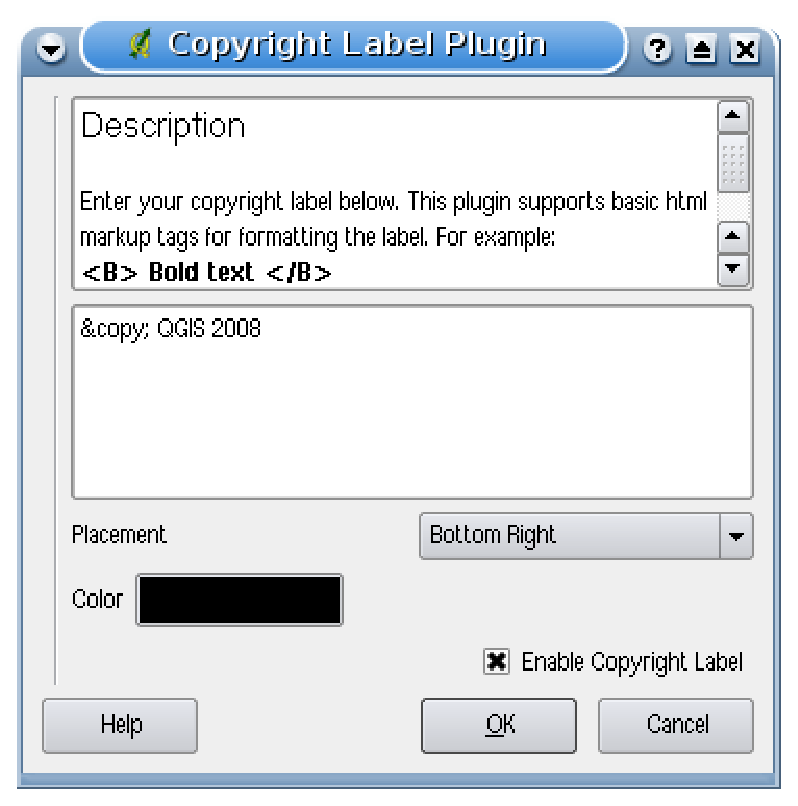
\includegraphics[clip=true, width=8cm]{copyright}
\end{center}  
\end{figure}

El título de este complemento puede dar lugar a confusión, ya que puede añadir cualquier texto aleatorio al mapa.

\begin{enumerate}
\item Asegúrese de que el complemento está cargado.
\item Pulse en la herramienta \textsl{Etiqueta de Copyright} en la barra de herramientas de complementos.
\item Introduzca el texto que desee colocar en el mapa. Puede usar HTML como en el ejemplo mostrado.
\item Seleccione el emplazamiento de la etiqueta en la casilla desplegable.
\item Asegúrese de que la casilla de verificación ``Activar etiqueta de copyright'' está marcada.
\item Pulse \textsl{Aceptar}
\end{enumerate}

En el ejemplo anterior, la primera línea está en negrita, la segunda (creada usando \textless br\textgreater) contiene un símbolo de copyright, seguido por el nombre de nuestra compañía en cursiva.

\subsubsection{Complemento flecha de Norte}

El complemento flecha de Norte coloca una sencilla flecha de Norte sobre la vista del mapa. Actualmente sólo hay un estilo disponible. Puede ajustar el ángulo de la flecha o dejar que QGIS establezca la dirección automáticamente. Si elige dejar que QGIS determine la dirección, averiguará lo mejor posible cómo se debe orientar la flecha.

En cuanto a la ubicación de la flecha, tiene cuatro opciones, correspondientes a las cuatro esquinas de la vista del mapa.

\begin{figure}[ht]
   \begin{center}
   \caption{Complemento flecha de Norte}\label{fig:north_arrow}\smallskip
   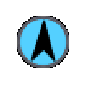
\includegraphics[clip=true, width=8cm]{north_arrow}
\end{center}  
\end{figure}

\subsubsection{Complemento barra de escala}
El complemento barra de escala añade una barra de escala sencilla a la vista del mapa. Puede controlar el estilo y la ubicación, así como el etiquetado de la barra.

QGIS sólo puede mostrar la escala en las mismas unidades que tenga el mapa. Por tanto, si sus capas están en metros no puede crear una barra de escala en pies. Del mismo modo, si está usando grados decimales no puede crear una barra de escala para mostrar las distancias en metros.

Para añadir una barra de escala:

\begin{enumerate}
\item Abra el diálogo del complemento pulsando en la herramienta \textsl{Barra de escala} en la barra de herramientas de complementos.
\item Seleccione la ubicación en la lista desplegable.
\item Seleccione el estilo.
\item Seleccione el color de la barra o use el negro predeterminado.
\item Establezca el tamaño de la barra y su etiqueta.
\item Asegúrese de que la casilla de verificación ``Activar barra de escala'' está marcada.
\item Opcionalmente puede elegir redondear a un número exacto cuando se redimensiona la vista del mapa.
\item Pulse \textsl{Aceptar} 
\end{enumerate} 

\begin{figure}[ht]
   \begin{center}
   \caption{Complemento barra de escala}\label{fig:scale_bar}\smallskip
   \includegraphics[clip=true, width=8cm]{scale_bar}
\end{center}  
\end{figure}

